%======================================================================
\NEWSEC
%======================================================================

\subsection{\ssDoubleMach}

\begin{frame}[fragile,label=ss-doublemach] 
\secframetitle{\ssDoubleMach}
\framesubtitle{Test problem specification}

\footnotesize
\begin{center}

\includegraphics[width=4.0in]{Images/DoubleMachAmr/doublemach-de-0000.png}
\end{center}

\begin{tabbing}
xxxxxxxxxxxxxxxxxxxxxxxxxxxxxxxx\=xxxxxxxxxxxxxxxxxxx\=\kill
\> \bluetext{Adiabatic index}: \' $\gamma = 1.4$. \\
\> \bluetext{Grid domain}: \' $0.0 < x < 4.0$, $0.0 < y < 1.0$ \\
\> \bluetext{Shock}: \' Mach 10, $v_s$ = 10.0, \\
\> \bluetext{Angle}: \' 30 degrees. \\
\> \bluetext{Pre-shock conditions}: \' $P = 1.0$, $\rho = 1.4$, $v = 0.0$ \\
\> \bluetext{Post-shock conditions}: \' $P = 116.5$, $\rho = 8$, $v = 8.25$ \\
\> \bluetext{Time limit}: \' $t = 0.25$.
\end{tabbing}
\end{frame}

%----------------------------------------------------------------------

\begin{frame}[fragile] 
\secframetitle{\ssDoubleMach}
\framesubtitle{\group{Domain} and \group{Stopping} criteria}
\begin{itemize}
\item \group{Domain}

\begin{itemize}
\item $0.0 < x < 4.0, 0.0 < y < 1.0$
\begin{semiverbatim}
\group{Domain} \{ 
   \parameter{lower} = [\valuetext{0.0}, \valuetext{0.0}];
   \parameter{upper} = [\valuetext{4.0}, \valuetext{1.0}];
\} 
\end{semiverbatim}
\end{itemize}
%
\item \group{Stopping} criteria
\begin{itemize}
%
\item $t=0.25$
%
\begin{semiverbatim}
\group{Stopping} \{ \variable{time} = \valuetext{0.25}; \} 
\end{semiverbatim}
%
\end{itemize}
\end{itemize}
\end{frame}

%----------------------------------------------------------------------

 \begin{frame}[fragile] 
 \secframetitle{\ssDoubleMach}
 \framesubtitle{\group{Initial} conditions}
\footnotesize
Complex initial conditions can be specified directly.

 \begin{itemize}
 \item To specify $x = a(x,y,z)$ in subregion $A$, else $x = b(x,y,z)$:
 \begin{tabbing}
 xxxxxxx\=\kill
\parameter{x} = \code{[} \> \valuetext{a(x,y,z)} \comment{\# (floating-point expression)}, \\
\>                         \valuetext{A(x,y,z)} \comment{\# (logical expression)}, \\
\>                         \valuetext{b(x,y,z)} \comment{\# (floating-point expression)} ];
 \end{tabbing}
 \item E.g. to specify ``$\rho = 8$ if $x \le 1/6 + 0.57735 y$, else $\rho = 1.4$'':
\begin{semiverbatim}
\group{Initial} \{
    \subgroup{density} \{
        \parameter{value} = [\valuetext{8.0}, \valuetext{(x <= 0.16667 + 0.57735*y)}, 
                 \valuetext{1.4}];  \}
\}
\end{semiverbatim}
\item Repeat with \subgroup{velocity\_x}, \subgroup{velocity\_y}, \subgroup{total\_energy}
 \end{itemize}
\end{frame}

%----------------------------------------------------------------------

\begin{frame}[fragile] 
\secframetitle{\ssDoubleMach}
\framesubtitle{\group{Initial} conditions}
\footnotesize
\begin{itemize}
\item Repeat with \subgroup{velocity\_x}, \subgroup{velocity\_y}, and \subgroup{total\_energy}
\begin{semiverbatim}
\group{Initial} \{
    \subgroup{velocity_x} \{
       \parameter{value} = [ \valuetext{8.25*0.8660253},
                        \valuetext{(x <= 0.16667 + 0.57735*y)},
                 \valuetext{0.0} ]; \}
    \subgroup{velocity_y} \{
       \parameter{value} = [\valuetext{-8.25*0.5},
                        \valuetext{(x <= 0.16667 + 0.57735*y)},
                 \valuetext{0.0}]; \}
    \subgroup{total_energy} \{
       \parameter{value} = [\valuetext{116.5 / (0.4 * 8.0) + 34.03125},
                        \valuetext{(x <= 0.16667 + 0.57735*y)}, 
                  \valuetext{1.0 / (0.4 * 1.4)}]; \}
 \}
\end{semiverbatim}
\end{itemize}
\end{frame}

%----------------------------------------------------------------------

 \begin{frame}[fragile] 
 \secframetitle{\ssDoubleMach}
 \framesubtitle{\group{Boundary} conditions}
\footnotesize
Complex boundary conditions can also be specified directly.

\begin{itemize}
\item General form:
 \begin{tabbing}
xxx\=xxx\=\kill
\group{Boundary} \{ \\
\>   \parameter{list} = [ \valuetext{"bc\_1"}, \valuetext{"bc\_2"}, \valuetext{"bc\_3"}, ... ];  \\
\\
\>   \subgroup{bc\_1} \{ \\
\>\>      \parameter{type} = \textit{\{} \valuetext{"inflow"}, \valuetext{"periodic"}, \valuetext{"outflow"}, \valuetext{"reflecting"} \textit{\}} \\
\>\>      \parameter{mask} = \valuetext{M(x,y,z,t)}; \comment{\# (logical expression)} \\
\>\>      \parameter{axis} = \textit{\{} \valuetext{"x"}, \valuetext{"y"}, \valuetext{"z"} \textit{\}} \\
\>\>      \parameter{face} = \textit{\{} \valuetext{"lower"}, \valuetext{"upper"}  \textit{\}} \\
\>\>      \parameter{field\_list} = [ \valuetext{velocity\_x} ]; \\
\>\>      \parameter{value} = \valuetext{M(x,y,z,t)}; \comment{\# (floating-point expression, inflow only)} \\
\>   \} \\
\>   \subgroup{bc\_2} \{ \ldots \} \\
\}
\end{tabbing}
\end{itemize}
\end{frame}
%  
%  % 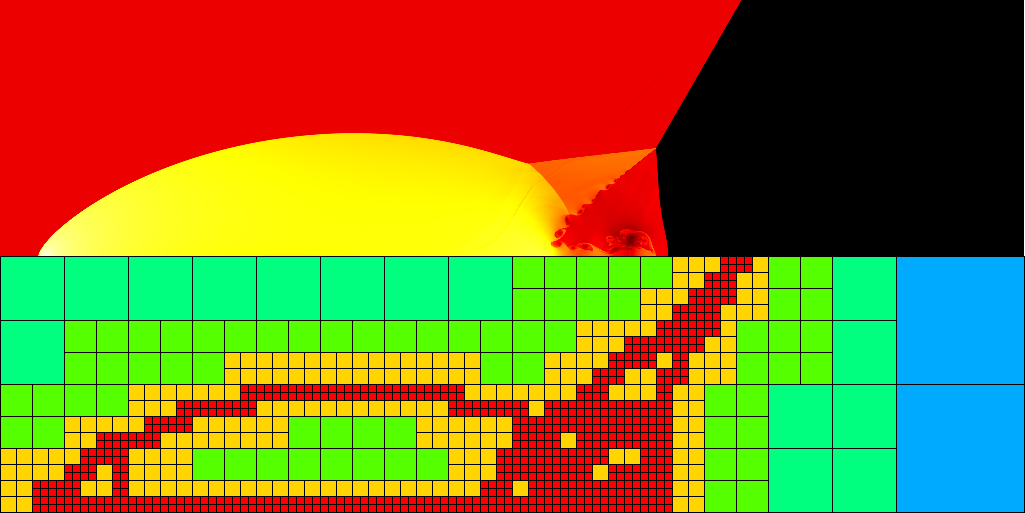
\includegraphics[width=4.0in]{Images/DoubleMachAmr/doublemach-0200.png}
%  % \ANIMATEGRAPHICS{width=4.5in}{20}{Images/DoubleMachAmr/doublemach-}{0000}{0307}
%  
%  
%  %    Boundary
%  %----------------------------------------------------------------------
%  
 \begin{frame}[fragile] 
 \secframetitle{\ssDoubleMach}
 \framesubtitle{\group{Boundary} conditions}
\footnotesize
\begin{semiverbatim}
 \group{Boundary} \{
    \variable{list} = [
            \valuetext{"OUT"},
            \valuetext{"REFLECT"},
            \valuetext{"DENSITY"},
            \valuetext{"VELOCITY_X"},
            \valuetext{"VELOCITY_Y"},
            \valuetext{"TOTAL_ENERGY}"
          ];
\}
\end{semiverbatim}
\end{frame}

%----------------------------------------------------------------------

 \begin{frame}[fragile] 
 \secframetitle{\ssDoubleMach}
 \framesubtitle{\group{Boundary} conditions: outflow and reflecting}
\footnotesize
\begin{semiverbatim}
 \group{Boundary} \{
    \subgroup{OUT} \{
       \variable{type} = \valuetext{"outflow"};
       \variable{mask} = [ (\variable{x} >= \valuetext{4.0}) || 
                (\variable{y} >= \valuetext{1.0} && (\variable{x} >= \valuetext{0.744017} + \valuetext{11.547}* \variable{t}))];
    \}
    \subgroup{REFLECT} \{
       \variable{type} = \valuetext{"reflecting"};
       \variable{axis} = \valuetext{"y"};
       \variable{face} = \valuetext{"lower"};
       \variable{mask} = (\variable{x} >= \valuetext{0.166667});
    \}
\} 
\end{semiverbatim}
\end{frame}

%----------------------------------------------------------------------

 \begin{frame}[fragile] 
 \secframetitle{\ssDoubleMach}
 \framesubtitle{\group{Boundary} conditions: \code{density}}
\footnotesize
\begin{semiverbatim}
\group{Boundary} \{
    \subgroup{DENSITY} \{
       \variable{type} = \valuetext{"inflow"};
       \variable{field_list} = \valuetext{"density"};
       \variable{value} = [ \valuetext{8.0}, 
                  ( (\variable{x} <= \valuetext{0.166667}) && (\variable{y} <= \valuetext{0.0}) ) ||
                    (\variable{x} <= \valuetext{0.0}) ||
                   ((\variable{x} <= \valuetext{0.744017} + \valuetext{11.547}*\variable{t)} && (\variable{y} >= \valuetext{1.0}))
               ];
    \}
\} 
\end{semiverbatim}
\end{frame}

%----------------------------------------------------------------------

 \begin{frame}[fragile] 
 \secframetitle{\ssDoubleMach}
 \framesubtitle{\group{Boundary} conditions: \code{velocity\_x}}
\footnotesize
\begin{semiverbatim}
\group{Boundary} \{
    \subgroup{VELOCITY_X} \{
       \variable{type} = \valuetext{"inflow"};
       \variable{field_list} = \valuetext{"velocity_x"};
       \variable{value} = [ \valuetext{8.25}*\valuetext{0.8660253},
                  ( (\variable{x} <= \valuetext{0.166667}) && (\variable{y} <= \valuetext{0.0}) ) ||
                    (\variable{x} <= \valuetext{0.0}) ||
                   ((\variable{x} <= \valuetext{0.744017} + \valuetext{11.547}*\variable{t)} && (\variable{y} >= \valuetext{1.0}))
               ];
    \}
\}
\end{semiverbatim}
\end{frame}

%----------------------------------------------------------------------

 \begin{frame}[fragile] 
 \secframetitle{\ssDoubleMach}
 \framesubtitle{\group{Boundary} conditions: \code{velocity\_y}}
\footnotesize
\begin{semiverbatim}
\group{Boundary} \{
    \subgroup{VELOCITY_Y} \{
       \variable{type} = \valuetext{"inflow"};
       \variable{field_list} = \valuetext{"velocity_y"};
       \variable{value} = [ -\valuetext{8.25}*\valuetext{0.5},
                  ( (\variable{x} <= \valuetext{0.166667}) && (\variable{y} <= \valuetext{0.0}) ) ||
                    (\variable{x} <= \valuetext{0.0}) ||
                   ((\variable{x} <= \valuetext{0.744017} + \valuetext{11.547}*\variable{t}) && (\variable{y} >= \valuetext{1.0}))
               ];
    \}
\}
\end{semiverbatim}
\end{frame}

%----------------------------------------------------------------------

 \begin{frame}[fragile] 
 \secframetitle{\ssDoubleMach}
 \framesubtitle{\group{Boundary} conditions: \code{total\_energy}}
\footnotesize
\begin{semiverbatim}
\group{Boundary} \{
    \subgroup{TOTAL_ENERGY} \{
       \variable{type} = \valuetext{"inflow"};
       \variable{field_list} = \valuetext{"total_energy"};
       \variable{value} = [ \valuetext{116.5} / (\valuetext{0.4} * \valuetext{8.0}) + \valuetext{34.03125},
                  ( (\variable{x} <= \valuetext{0.166667}) && (\variable{y} <= \valuetext{0.0}) ) ||
                    (\variable{x} <= \valuetext{0.0}) ||
                   ((\variable{x} <= \valuetext{0.744017} + \valuetext{11.547}*\variable{t)} && (\variable{y} >= \valuetext{1.0}))
               ];
    \}
\}
\end{semiverbatim}
\end{frame}

%----------------------------------------------------------------------

 \begin{frame}[fragile] 
 \secframetitle{\ssDoubleMach}
 \framesubtitle{Discretization: \group{Mesh} (array) and \group{Adapt} (octrees)}
\footnotesize
%    Stopping
% \end{itemize}


\begin{semiverbatim}
\group{Mesh} \{
   \variable{root_rank} = \valuetext{2};
   \variable{root_size} = [\valuetext{96},\valuetext{24}];
   \variable{root_blocks} = [\valuetext{4},\valuetext{1}]; \comment{\# $24^2$ block size}
\}
\group{Adapt} \{
   \variable{max_level} = \valuetext{5}; 
   \variable{list} = [\valuetext{"SLOPE"}];
   \subgroup{SLOPE} \{
      \variable{type} = \valuetext{"slope"};
      \variable{field_list} = [\valuetext{"density"}];
      \variable{min_refine}  = \valuetext{5.0};
      \variable{max_coarsen} = \valuetext{2.0};
   \}
\}
\end{semiverbatim}
\end{frame}

%----------------------------------------------------------------------

 \begin{frame}[fragile] 
 \secframetitle{\ssDoubleMach}
 \framesubtitle{\group{Field} parameters}
\footnotesize
% 
% 
\begin{semiverbatim}
\group{Field} \{
   \variable{gamma} = \valuetext{1.4};
   \variable{list} = [
      \valuetext{"density"},        
      \valuetext{"velocity_x"},
      \valuetext{"velocity_y"},
      \valuetext{"total_energy"},
      \valuetext{"internal_energy"},
      \valuetext{"pressure"} ];
   \variable{ghost_depth} = \valuetext{4}; \comment{\# currently required by interpolation}
\}
\end{semiverbatim}
\end{frame}

%----------------------------------------------------------------------

 \begin{frame}[fragile] 
 \secframetitle{\ssDoubleMach}
 \framesubtitle{\group{Method} parameters}
\footnotesize
\begin{semiverbatim}
\group{Method} \{
   \variable{list} = [\valuetext{"ppm"}];

   \subgroup{ppm} \{
      \variable{diffusion}   = \valuetext{true};
      \variable{flattening}  = \valuetext{3};
      \variable{steepening}  = \valuetext{true};
      \variable{dual_energy} = \valuetext{false};
   \}
   \variable{courant}   = \valuetext{0.8};
\}
\end{semiverbatim}
\end{frame}

%----------------------------------------------------------------------

 \begin{frame}[fragile] 
 \secframetitle{\ssDoubleMach}
 \framesubtitle{\group{Output} parameters}
%\footnotesize
We wish to output
\begin{itemize}
\item HDF5 files of all data
\item density as an image
\item mesh refinement as an image
\end{itemize}

\begin{semiverbatim}
\group{Output} \{ 
   \variable{list} = [\valuetext{"hdf5"},\valuetext{"de_image"},\valuetext{"mesh_image"}];
\}
\end{semiverbatim}
\end{frame}

%----------------------------------------------------------------------

 \begin{frame}[fragile] 
 \secframetitle{\ssDoubleMach}
 \framesubtitle{\group{Output} data as HDF5}
\footnotesize
\begin{semiverbatim}
\group{Output} \{ 
   \subgroup{hdf5} \{
      \variable{type} = \valuetext{"data"};
      \variable{name} = [\valuetext{"doublemach-p%02d-c%04d.h5"}, \valuetext{"proc"},\valuetext{"count"}]; 
      \keyword{include} \valuetext{"input/schedule_cycle_25.incl"}
   \}
\}
\end{semiverbatim}
\end{frame}

%----------------------------------------------------------------------

 \begin{frame}[fragile] 
 \secframetitle{\ssDoubleMach}
 \framesubtitle{\group{Output} image of density}
\footnotesize
\begin{semiverbatim}
\group{Output} \{ 
   \subgroup{de_image} \{
      \variable{type} = \valuetext{"image"};
      \variable{name} = [\valuetext{"doublemach-de-%04d.png"}, \valuetext{"count"}]; 
      \variable{field_list} = [\valuetext{"density"}];
      \variable{image_size} = [\valuetext{1024},\valuetext{256}];
      \keyword{include} \valuetext{"input/schedule_cycle_25.incl"}
      \keyword{include} \valuetext{"input/colormap_blackbody.incl"}
   \}
\}
\end{semiverbatim}
\end{frame}

%----------------------------------------------------------------------

 \begin{frame}[fragile] 
 \secframetitle{\ssDoubleMach}
 \framesubtitle{\group{Output} image of mesh hierarchy}
\footnotesize

\begin{semiverbatim}
\group{Output} \{ 
    \subgroup{mesh_image} \{
        \variable{type}     = \valuetext{"image"};
        \variable{name} = [\valuetext{"doublemach-mesh-%04d.png"}, \valuetext{"count"}];
        \variable{image_type}  = \valuetext{"mesh"};
        \variable{image_reduce_type} = \valuetext{"max"};
        \variable{image_size} = [\valuetext{1025},\valuetext{257}];
        \keyword{include} \valuetext{"input/schedule_cycle_25.incl"}
        \variable{image_specify_bounds} = \valuetext{true};
        \variable{image_min} = \valuetext{0.0};
        \variable{image_max} = \valuetext{6.0};
        \keyword{include} \valuetext{"input/colormap_rainbow.incl"}
      \}
\}
\end{semiverbatim}
\end{frame}

%----------------------------------------------------------------------

\begin{frame}[fragile]
\secframetitle{\ssDoubleMach}
\footnotesize
\begin{center}
\ANIMATEGRAPHICS{width=4.0in}{20}{Images/DoubleMachAmr/doublemach-0}{000}{272}
\end{center}
\end{frame}

